% This file was created by tikzplotlib v0.9.9.
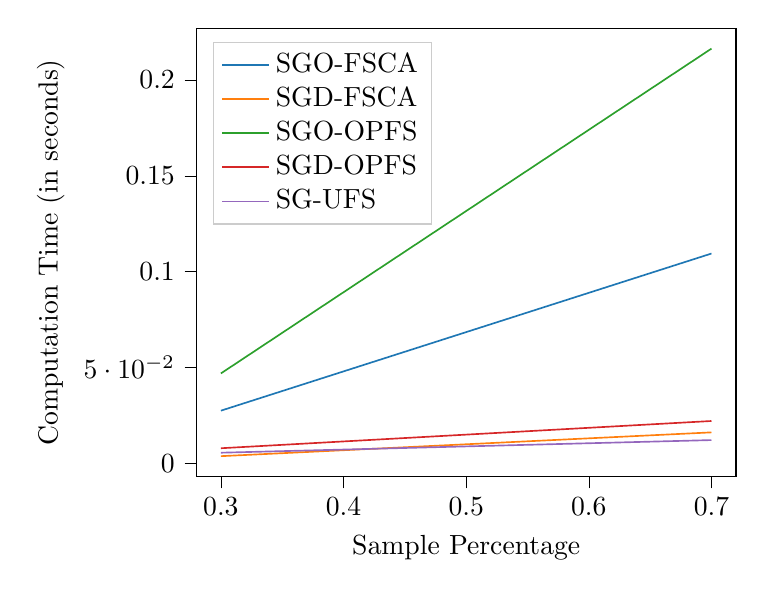
\begin{tikzpicture}

\definecolor{color0}{rgb}{0.12156862745098,0.466666666666667,0.705882352941177}
\definecolor{color1}{rgb}{1,0.498039215686275,0.0549019607843137}
\definecolor{color2}{rgb}{0.172549019607843,0.627450980392157,0.172549019607843}
\definecolor{color3}{rgb}{0.83921568627451,0.152941176470588,0.156862745098039}
\definecolor{color4}{rgb}{0.580392156862745,0.403921568627451,0.741176470588235}

\begin{axis}[
legend cell align={left},
legend style={
  fill opacity=0.8,
  draw opacity=1,
  text opacity=1,
  at={(0.03,0.97)},
  anchor=north west,
  draw=white!80!black
},
tick align=outside,
tick pos=left,
x grid style={white!69.0196078431373!black},
xlabel={Sample Percentage},
xmin=0.28, xmax=0.72,
xtick style={color=black},
y grid style={white!69.0196078431373!black},
ylabel={Computation Time (in seconds)},
ymin=-0.00684645, ymax=0.22704545,
ytick style={color=black}
]
\addplot [semithick, color0]
table {%
0.3 0.027519
0.7 0.109502
};
\addlegendentry{SGO-FSCA}
\addplot [semithick, color1]
table {%
0.3 0.003785
0.7 0.016198
};
\addlegendentry{SGD-FSCA}
\addplot [semithick, color2]
table {%
0.3 0.046948
0.7 0.216414
};
\addlegendentry{SGO-OPFS}
\addplot [semithick, color3]
table {%
0.3 0.00792
0.7 0.022133
};
\addlegendentry{SGD-OPFS}
\addplot [semithick, color4]
table {%
0.3 0.005586
0.7 0.012176
};
\addlegendentry{SG-UFS}
\end{axis}

\end{tikzpicture}
